\documentclass[11pt,a4paper]{article}

\usepackage[margin=2.5cm]{geometry}
\usepackage{amsmath,amssymb,amsthm}
\usepackage{enumitem}
\usepackage{hyperref}
\usepackage{tikz}
\usetikzlibrary{arrows.meta,positioning,trees,calc,fit,shapes.geometric,backgrounds}

% Haskell-style code listings
\usepackage{listings}
\lstdefinelanguage{FunctionalPseudo}{
  morekeywords={data,type,where,let,in,if,then,else,case,of,do,
    module,import,class,instance,deriving,forall,newtype},
  morekeywords=[2]{Int,Bool,True,False,Maybe,Just,Nothing,
    IntSet,IntMap,Set,Map,Forest,Tree,IO,IORef,MVar,
    Strategy,Eval,Par},
  morekeywords=[3]{filter,map,concatMap,minimum,all,any,not,
    unfoldForest,flatten,parMap,parBuffer,rpar,rseq,
    readIORef,writeIORef,modifyIORef},
  sensitive=true,
  morecomment=[l]{--},
  morecomment=[s]{\{-}{-\}},
  morestring=[b]",
  literate={->}{{$\to$}}2 {=>}{{$\Rightarrow$}}2
           {<-}{{$\leftarrow$}}2
           {::}{{$\mathrel{::}$}}2
           {\\}{{$\lambda$}}1
           {forall}{{$\forall$}}1
           {/=}{{$\neq$}}1
           {<=}{{$\le$}}1
           {>=}{{$\ge$}}1
           {&&}{{$\wedge$}}1
           {||}{{$\vee$}}1
           {++}{{$\mathbin{+\mkern-6mu+}$}}1
           {...}{{$\ldots$}}1
}
\lstset{
  language=FunctionalPseudo,
  basicstyle=\small\ttfamily,
  keywordstyle=\bfseries,
  keywordstyle=[2]\itshape,
  keywordstyle=[3]\upshape,
  commentstyle=\itshape\color[rgb]{0.4,0.4,0.4},
  columns=flexible,
  keepspaces=true,
  showstringspaces=false,
  xleftmargin=1em,
  frame=single,
  framesep=4pt,
  aboveskip=8pt,
  belowskip=8pt,
  escapeinside={(*@}{@*)},
  mathescape=false,
}

\newtheorem{theorem}{Theorem}[section]
\newtheorem{lemma}[theorem]{Lemma}
\newtheorem{proposition}[theorem]{Proposition}
\newtheorem{corollary}[theorem]{Corollary}
\theoremstyle{definition}
\newtheorem{definition}[theorem]{Definition}
\newtheorem{remark}[theorem]{Remark}

% Notation shortcuts
\newcommand{\Ful}{\mathrm{Ful}}
\newcommand{\DualTri}{\mathrm{DualTri}}
\newcommand{\CanRed}{\mathrm{canonRed}}
\newcommand{\CanOrd}{\mathrm{CanOrd}}

\title{Buckygen as Functional Pseudocode\\[6pt]
\large A specification for Haskell and C++ implementations}
\author{}
\date{\today}

\begin{document}
\maketitle

\begin{abstract}
We present the buckygen fullerene generation
algorithm~\cite{brinkmann_12} as functional pseudocode, using
Haskell-flavoured notation.  The algorithm is an instance of McKay's
canonical construction path method~\cite{mckay_98}: the set of all
fullerenes forms a \emph{canonical search forest} under the canonical
parent relation, and the generation is a pruned unfolding of this
forest.  This formulation makes the algebraic structure
explicit---independence of subtrees, purity of all core functions, and
composability of pruning predicates---enabling both parallel evaluation
and branch-and-bound extensions without changing the algorithm's
semantics.
\end{abstract}

\tableofcontents
\newpage

%======================================================================
\section{The Generation Problem}
\label{sec:problem}
%======================================================================

%----------------------------------------------------------------------
\subsection{Formal definition}
%----------------------------------------------------------------------

\begin{definition}[Fullerene]
A \textbf{fullerene} on $n$ vertices is a 3-connected cubic planar
graph in which every face is a pentagon or hexagon.  By Euler's formula
it has exactly $12$ pentagons and $n/2 - 10$ hexagons.
\end{definition}

\begin{definition}[Dual fullerene]
The \textbf{dual} of a fullerene is a triangulation in which every
vertex has degree~5 or~6, with exactly $12$ degree-5 vertices.  The
dual has $n/2 + 2$ vertices and $3(n/2 + 2) - 6$ edges.  Buckygen
works entirely in this dual representation.
\end{definition}

The generation problem is:
\[
  \text{Compute } \Ful(n) \;=\; \DualTri(n/2+2,\,\{5,6\})\,\big/\,{\cong}
\]
i.e.\ enumerate one representative from each isomorphism class of dual
fullerene triangulations with $n/2 + 2$ vertices, all of degree 5 or~6.

%----------------------------------------------------------------------
\subsection{The canonical parent forest}
\label{sec:forest}
%----------------------------------------------------------------------

The construction theorem~\cite{hasheminezhad_08} gives a set of
\emph{expansion} operations (Section~\ref{sec:expansion-types}) whose
inverses are \emph{reductions}.  Among all reductions of a dual
fullerene~$G$, a canonical ordering (Section~\ref{sec:canonical-ord})
selects a unique \textbf{canonical reduction}.  Applying it yields the
\textbf{canonical parent} of~$G$.

\begin{definition}[Canonical parent forest]
\label{def:forest}
Define a directed graph on the set of all dual fullerenes (up to
isomorphism) by $G \to \mathrm{parent}(G)$.  This graph is a
\textbf{forest} whose roots are the irreducible dual fullerenes:
\begin{itemize}[nosep]
  \item $C_{20}$ (the dodecahedron): $12$ dual vertices, all degree~5.
  \item $C_{28}(T_d)$: $16$ dual vertices.
  \item $C_{30}(D_{5h})$: $17$ dual vertices (smallest type-$(5,0)$ nanotube).
\end{itemize}
\end{definition}

\begin{theorem}[Recursive structure]
\label{thm:recursive}
The set $\Ful(n)$ equals the set of all leaves and internal nodes at
depth $d$ in the canonical parent forest, where $d$ is determined by
the target vertex count.  Each subtree rooted at an irreducible
fullerene is independent: no cross-tree communication is needed, and
results are collected by list concatenation (the free monoid).
\end{theorem}

This is an instance of McKay's canonical construction path
method~\cite{mckay_98}: generate by canonical expansion, reject
non-canonical children.

\begin{figure}[ht]
\centering
% The Canonical Parent Forest
% Three independent trees rooted at the irreducible fullerenes.
% Each node is a dual fullerene; edges are canonical expansions.
% Subtrees are independent (no cross-tree edges).
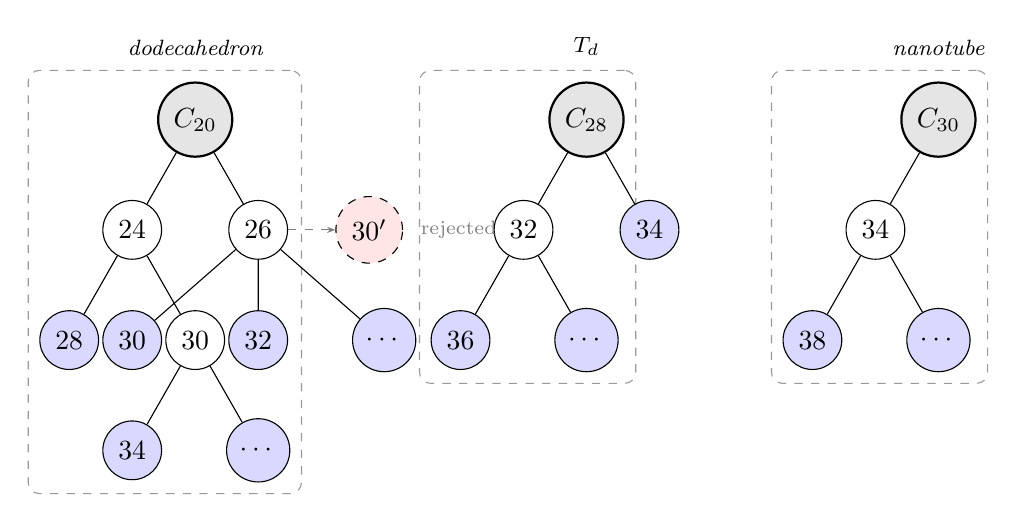
\begin{tikzpicture}[
    % --- Node styles ---
    root/.style={draw, circle, thick, minimum size=8mm, fill=black!10},
    inner/.style={draw, circle, minimum size=6mm, fill=white},
    leaf/.style={draw, circle, minimum size=6mm, fill=blue!15},
    rejected/.style={draw, circle, minimum size=5mm, fill=red!10, dashed},
    % --- Edge styles ---
    expansion/.style={-{Stealth[length=4pt]}, thick},
    rejected edge/.style={-{Stealth[length=3pt]}, dashed, gray},
    % --- Layout ---
    level distance=14mm,
    sibling distance=16mm,
]

% === Tree 1: rooted at C20 (the main tree) ===
% C20 has 12 dual vertices (all degree-5, the icosahedron).
% L_0 adds 2 dual verts => +4 primal verts => C24.
% L_1 / B_{0,0} add 3 dual verts => +6 primal verts => C26.
\node[root] (c20) {$C_{20}$}
  child {
    node[inner] (c24) {$24$}
    % From C24: L_0 => C28, L_1/B00 => C30, ...
    child { node[leaf] (c28a) {$28$} }
    child { node[inner] (c30a) {$30$}
      child { node[leaf] (c34a) {$34$} }
      child { node[leaf] (c34b) {$\cdots$} }
    }
  }
  child {
    node[inner] (c26) {$26$}
    % From C26: L_0 => C30, L_1/B00 => C32, ...
    child { node[leaf] (c30b) {$30$} }
    child { node[leaf] (c32a) {$32$} }
    child { node[leaf] (c32b) {$\cdots$} }
  };

% === Tree 2: rooted at C28(Td) ===
% C28 has 16 dual vertices.
% L_0 => C32, L_1/B00 => C34, ...
\node[root, right=40mm of c20] (c28) {$C_{28}$}
  child {
    node[inner] (c32c) {$32$}
    child { node[leaf] (c36a) {$36$} }
    child { node[leaf] (c36b) {$\cdots$} }
  }
  child {
    node[leaf] (c34c) {$34$}
  };

% === Tree 3: rooted at C30(D5h), the nanotube family ===
% C30 has 17 dual vertices.
% F expansion adds 5 dual verts => +10 primal verts => C40.
% L/B expansions also possible: L_0 => C34, etc.
\node[root, right=35mm of c28] (c30) {$C_{30}$}
  child {
    node[inner] (c34d) {$34$}
    child { node[leaf] (c38a) {$38$} }
    child { node[leaf] (c38b) {$\cdots$} }
  }
  child[missing] {};

% --- Annotations ---
% Label the trees
\node[above=2mm of c20, font=\footnotesize\itshape] {dodecahedron};
\node[above=2mm of c28, font=\footnotesize\itshape] {$T_d$};
\node[above=2mm of c30, font=\footnotesize\itshape] {nanotube};

% Show independence: dashed box around each tree
\begin{scope}[on background layer]
  \node[fit=(c20)(c28a)(c34b), draw=black!40, dashed,
        rounded corners=4pt, inner sep=4pt] {};
  \node[fit=(c28)(c36a)(c36b), draw=black!40, dashed,
        rounded corners=4pt, inner sep=4pt] {};
  \node[fit=(c30)(c38a)(c38b), draw=black!40, dashed,
        rounded corners=4pt, inner sep=4pt] {};
\end{scope}

% Rejected (non-canonical) child shown to the side
\node[rejected, right=6mm of c26] (rej) {$30'$};
\draw[rejected edge] (c26) -- (rej);
\node[right=1mm of rej, font=\scriptsize, gray] {rejected};

\end{tikzpicture}
\caption{The canonical parent forest.  Roots are the three irreducible
fullerenes.  Numbers indicate primal vertex counts $n$ (always even;
the dual has $n/2+2$ vertices).  $L_0$ adds $4$ to $n$; $L_1$ and
$B_{0,0}$ add $6$.  Solid nodes are canonical children; the dashed
node $30'$ is a non-canonical expansion (rejected by
\texttt{isCanonical}).  Each dashed box is an independent subtree
that can be evaluated in parallel.}
\label{fig:forest}
\end{figure}

%======================================================================
\section{Core Types}
\label{sec:types}
%======================================================================

All types are pure (no mutable state).  The notation is
Haskell-flavoured but intended as a mathematical specification.

%----------------------------------------------------------------------
\subsection{Dual graph representation}
%----------------------------------------------------------------------

\begin{lstlisting}
data DualGraph = DG
  { numVertices :: Int                  -- |V|
  , neighbours  :: IntMap [Vertex]      -- adjacency: circular order
  , degree5     :: [Vertex]             -- the 12 five-vertices (sorted)
  }

type Vertex = Int
type Edge   = (Vertex, Vertex)          -- directed: (start, end)
\end{lstlisting}

The adjacency list for each vertex stores neighbours in \emph{cyclic
planar order} (clockwise in the chosen embedding).  This is essential
for the patch-replacement operations.

%----------------------------------------------------------------------
\subsection{Expansion and reduction}
\label{sec:expansion-types}
%----------------------------------------------------------------------

\begin{lstlisting}
data ExpKind
  = L Int           -- L_i: straight, parameter i >= 0
  | B Int Int       -- B_{i,j}: bent, parameters i,j >= 0, i+j > 0
  | F               -- nanotube ring addition

data Expansion = Exp
  { expKind   :: ExpKind
  , startEdge :: Edge       -- directed edge starting the central path
  , direction :: Dir        -- left/right orientation of the patch
  }

data Reduction = Red
  { redKind   :: ExpKind
  , startEdge :: Edge
  , direction :: Dir
  }

data Dir = DLeft | DRight
\end{lstlisting}

Every expansion has a unique inverse reduction.  Applying an
expansion of kind $L_i$ adds $i+2$ vertices; $B_{i,j}$ adds $i+j+3$
vertices; $F$ adds $5$ vertices (one ring of the nanotube).

\begin{figure}[ht]
\centering
% Expansion operations: L (straight) and B (bent)
% Shows the central path between two 5-vertices and the patch replacement.
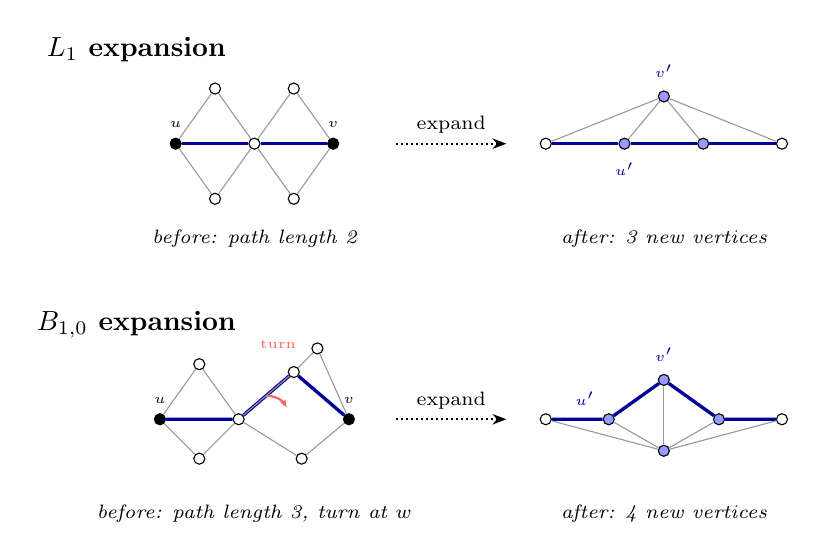
\begin{tikzpicture}[
    % --- Vertex styles ---
    deg5/.style={draw, circle, fill=black, minimum size=4pt, inner sep=0pt,
                 label={[font=\tiny]above:#1}},
    deg6/.style={draw, circle, fill=white, minimum size=4pt, inner sep=0pt},
    newvert/.style={draw, circle, fill=blue!40, minimum size=4pt, inner sep=0pt},
    % --- Edge styles ---
    path edge/.style={very thick, blue!60!black},
    mesh edge/.style={thin, black!40},
    % --- Arrow between before/after ---
    transforms to/.style={-{Stealth[length=5pt]}, thick, densely dotted},
]

% ============================================================
% L_1 expansion: straight path of length 2 between two 5-vertices
% ============================================================
\node[font=\bfseries] at (-1.5, 1.2) {$L_1$ expansion};

% --- Before: path u--w--v, where u,v are degree-5 ---
\begin{scope}[shift={(0,0)}]
  \node[font=\scriptsize\itshape] at (0, -1.2) {before: path length 2};

  % The central path: u -- w -- v (straight, no turn)
  \node[deg5={$u$}]  (Lu) at (-1, 0) {};     % 5-vertex (start)
  \node[deg6]        (Lw) at ( 0, 0) {};     % 6-vertex (interior)
  \node[deg5={$v$}]  (Lv) at ( 1, 0) {};     % 5-vertex (end)

  % Mesh edges (surrounding triangulation, schematic)
  \node[deg6] (La) at (-0.5,  0.7) {};
  \node[deg6] (Lb) at ( 0.5,  0.7) {};
  \node[deg6] (Lc) at (-0.5, -0.7) {};
  \node[deg6] (Ld) at ( 0.5, -0.7) {};

  % Central path edges
  \draw[path edge] (Lu) -- (Lw) -- (Lv);
  % Surrounding mesh
  \foreach \a/\b in {Lu/La, La/Lw, Lw/Lb, Lb/Lv, Lu/Lc, Lc/Lw, Lw/Ld, Ld/Lv}
    \draw[mesh edge] (\a) -- (\b);
\end{scope}

% --- Arrow ---
\draw[transforms to] (1.8, 0) -- node[above, font=\scriptsize] {expand} (3.2, 0);

% --- After: 3 new vertices inserted, u',v' become the new 5-vertices ---
\begin{scope}[shift={(5.2,0)}]
  \node[font=\scriptsize\itshape] at (0, -1.2) {after: 3 new vertices};

  % Old endpoints become degree-6
  \node[deg6]         (Lu2) at (-1.5, 0) {};
  \node[deg6]         (Lv2) at ( 1.5, 0) {};

  % New vertices (the inserted patch)
  \node[newvert] (Ln1) at (-0.5, 0) {};        % new degree-5 (u')
  \node[newvert] (Ln2) at ( 0.5, 0) {};        % new interior
  \node[newvert] (Ln3) at ( 0,   0.6) {};      % new degree-5 (v')

  % Mark the new 5-vertices
  \node[font=\tiny, blue!60!black, below=1pt of Ln1] {$u'$};
  \node[font=\tiny, blue!60!black, above=1pt of Ln3] {$v'$};

  % Edges in expanded patch
  \draw[path edge] (Lu2) -- (Ln1) -- (Ln2) -- (Lv2);
  \draw[mesh edge] (Ln1) -- (Ln3) -- (Ln2);
  \draw[mesh edge] (Lu2) -- (Ln3) -- (Lv2);
\end{scope}

% ============================================================
% B_{1,0} expansion: bent path with a turn
% ============================================================
\begin{scope}[shift={(0, -3.5)}]
\node[font=\bfseries] at (-1.5, 1.2) {$B_{1,0}$ expansion};

% --- Before: path u--w--x--v with a turn at w ---
\begin{scope}
  \node[font=\scriptsize\itshape] at (0, -1.2) {before: path length 3, turn at $w$};

  \node[deg5={$u$}]  (Bu) at (-1.2,  0) {};
  \node[deg6]        (Bw) at (-0.2,  0) {};   % the turn vertex
  \node[deg6]        (Bx) at ( 0.5,  0.6) {}; % path bends here
  \node[deg5={$v$}]  (Bv) at ( 1.2,  0) {};

  % Central path (bent: goes u--w then turns up to x then to v)
  \draw[path edge] (Bu) -- (Bw) -- (Bx) -- (Bv);
  % Mark the turn
  \draw[thick, red!60, -{Stealth[length=3pt]}]
    ($(Bw)!0.5!(Bx)$) arc[start angle=90, end angle=30, radius=3mm];
  \node[font=\tiny, red!60] at (0.3, 0.95) {turn};

  % Surrounding mesh (schematic)
  \node[deg6] (Ba) at (-0.7,  0.7) {};
  \node[deg6] (Bb) at ( 0.8,  0.9) {};
  \node[deg6] (Bc) at (-0.7, -0.5) {};
  \node[deg6] (Bd) at ( 0.6, -0.5) {};
  \foreach \a/\b in {Bu/Ba, Ba/Bw, Bw/Bx, Bx/Bb, Bv/Bb, Bu/Bc, Bc/Bw, Bw/Bd, Bd/Bv}
    \draw[mesh edge] (\a) -- (\b);
\end{scope}

% --- Arrow ---
\draw[transforms to] (1.8, 0) -- node[above, font=\scriptsize] {expand} (3.2, 0);

% --- After ---
\begin{scope}[shift={(5.2,0)}]
  \node[font=\scriptsize\itshape] at (0, -1.2) {after: 4 new vertices};

  \node[deg6]    (Bu2) at (-1.5, 0) {};
  \node[deg6]    (Bv2) at ( 1.5, 0) {};
  \node[newvert] (Bn1) at (-0.7, 0) {};
  \node[newvert] (Bn2) at ( 0,   0.5) {};
  \node[newvert] (Bn3) at ( 0.7, 0) {};
  \node[newvert] (Bn4) at ( 0,  -0.4) {};

  \node[font=\tiny, blue!60!black, above left=0pt of Bn1] {$u'$};
  \node[font=\tiny, blue!60!black, above=1pt of Bn2] {$v'$};

  \draw[path edge] (Bu2) -- (Bn1) -- (Bn2) -- (Bn3) -- (Bv2);
  \draw[mesh edge] (Bn1) -- (Bn4) -- (Bn3);
  \draw[mesh edge] (Bu2) -- (Bn4) -- (Bv2);
  \draw[mesh edge] (Bn2) -- (Bn4);
\end{scope}

\end{scope}

\end{tikzpicture}
\caption{Expansion operations.  Black dots are degree-5 vertices; white
dots are degree-6; blue dots are newly created vertices.  The thick
blue path connects the two 5-vertices.  $L_1$ is \emph{straight}
(no turn); $B_{1,0}$ is \emph{bent} (the path turns at vertex~$w$).
After expansion, the old 5-vertices become degree-6 and two new
5-vertices ($u'$, $v'$) appear.}
\label{fig:expansions}
\end{figure}

%----------------------------------------------------------------------
\subsection{Canonical ordering}
\label{sec:canonical-ord}
%----------------------------------------------------------------------

\begin{lstlisting}
type CanOrd = (Int, Int, [Int], [Int], [Int], BFSCode)

data BFSCode = BFS [Int]  -- BFS-based canonical labelling
  deriving (Eq, Ord)
\end{lstlisting}

The 6-tuple is used to lexicographically order all reductions of a
graph.  Entries are computed lazily: $x_5$ (the expensive BFS code) is
only evaluated when $(x_0, \ldots, x_4)$ leaves a tie.

\begin{center}
\begin{tabular}{clcl}
Entry & Meaning & Cost & Discriminating power \\
\hline
$x_0$ & Path length (distance between 5-vertices) & $O(1)$ & High \\
$x_1$ & $-(\text{longest straight segment})$ & $O(1)$ & Medium \\
$x_2$ & Degree string, small neighbourhood & $O(1)$ & Good \\
$x_3$ & Degree string, medium neighbourhood & $O(1)$ & Good \\
$x_4$ & Degree string, larger neighbourhood & $O(1)$ & Good \\
$x_5$ & Full BFS canonical form & $O(n)$ & Perfect \\
\end{tabular}
\end{center}

%======================================================================
\section{The Algorithm as Tree Unfold}
\label{sec:unfold}
%======================================================================

The entire generation is a \emph{filtered unfolding} of the canonical
parent forest.

%----------------------------------------------------------------------
\subsection{Top-level: forest generation}
%----------------------------------------------------------------------

\begin{lstlisting}
generationForest :: Int -> Forest DualGraph
generationForest nTarget = unfoldForest step (seeds nTarget)
  where
    step g = (g, canonicalChildren nTarget g)

seeds :: Int -> [DualGraph]
seeds nTarget =
    [c20]
    ++ [c28 | nTarget >= 28]
    ++ [c30 | nTarget >= 30]
  where
    c20 = decodePlanarCode "..."   -- the dodecahedron
    c28 = decodePlanarCode "..."   -- C_28(T_d)
    c30 = decodePlanarCode "..."   -- C_30(D_5h)
\end{lstlisting}

The \texttt{unfoldForest} function from \texttt{Data.Tree} generates a
lazy forest: each node is labelled with a dual graph, and its children
are all canonical expansions.

%----------------------------------------------------------------------
\subsection{Collecting results}
%----------------------------------------------------------------------

\begin{lstlisting}
fullerenes :: Int -> [DualGraph]
fullerenes nTarget =
    concatMap flatten (generationForest nTarget)
  & filter (\g -> numVertices g == nTarget)
\end{lstlisting}

Because results are collected via \texttt{concatMap} (list
concatenation, the free monoid), the order of subtree evaluation is
irrelevant.

%----------------------------------------------------------------------
\subsection{Canonical children}
%----------------------------------------------------------------------

\begin{lstlisting}
canonicalChildren :: Int -> DualGraph -> [DualGraph]
canonicalChildren nTarget g
  | numVertices g >= nTarget = []   -- already at target size
  | otherwise =
      [ g'
      | e <- expansions (maxLength g nTarget) g
      , let g' = applyExpansion e g
      , numVertices g' <= nTarget
      , isCanonical e g'
      ]
\end{lstlisting}

This is the heart of the algorithm.  It composes five pure functions,
detailed in Section~\ref{sec:decomposition}.

%======================================================================
\section{Decomposition of \texttt{canonicalChildren}}
\label{sec:decomposition}
%======================================================================

The function \texttt{canonicalChildren} decomposes into five pure
functions that form a pipeline (Figure~\ref{fig:pipeline}).  Each can
be understood, tested, and optimised independently.

\begin{figure}[ht]
\centering
% The five-function pipeline inside canonicalChildren.
% Data flows left to right: graph -> bound -> expansions -> apply -> test -> children.
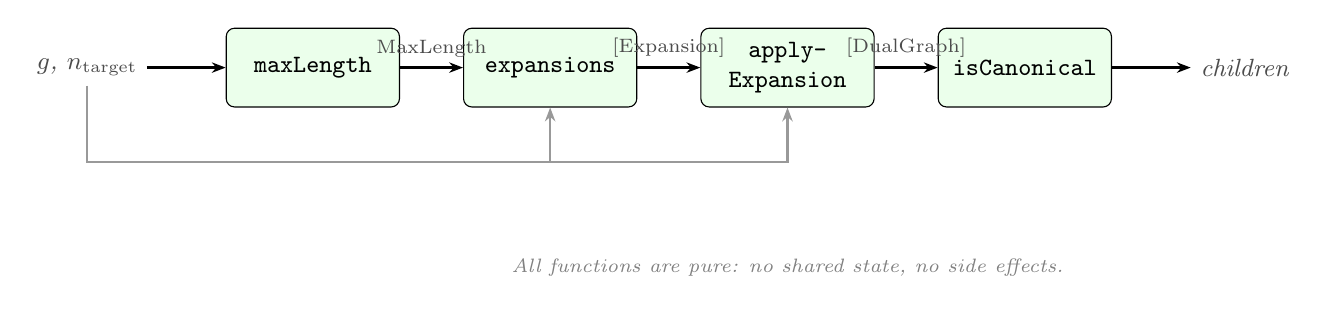
\begin{tikzpicture}[
    % --- Box styles ---
    func/.style={draw, rounded corners=3pt, minimum height=10mm,
                 minimum width=22mm, align=center, font=\small\ttfamily},
    pure/.style={func, fill=green!8},
    data/.style={font=\small\itshape, text=black!70},
    % --- Arrow style ---
    flow/.style={-{Stealth[length=5pt]}, thick},
]

% === The five functions as boxes ===
\node[pure]                  (bound)  {maxLength};
\node[pure, right=8mm of bound]   (expand) {expansions};
\node[pure, right=8mm of expand]  (apply)  {apply-\\Expansion};
\node[pure, right=8mm of apply]   (test)   {isCanonical};

% === Input on the left ===
\node[data, left=10mm of bound] (input) {$g$, $n_{\mathrm{target}}$};

% === Output on the right ===
\node[data, right=10mm of test] (output) {children};

% === Data flow arrows with labels ===
\draw[flow] (input) -- (bound);
\draw[flow] (bound) -- node[above, data, font=\scriptsize] {MaxLength} (expand);
\draw[flow] (expand) -- node[above, data, font=\scriptsize] {[Expansion]} (apply);
\draw[flow] (apply) -- node[above, data, font=\scriptsize] {[DualGraph]} (test);
\draw[flow] (test) -- (output);

% === The graph g is also fed to expand, apply, test (shown as curved arrows below) ===
% g feeds into all stages
\coordinate (gfeed) at ($(input)+(0,-12mm)$);
\draw[flow, black!40] (input.south) |- (gfeed) -| (expand.south);
\draw[flow, black!40] (gfeed) -| (apply.south);

% === Label: all functions are pure ===
\node[below=18mm of apply, font=\scriptsize\itshape, text=black!50]
  {All functions are pure: no shared state, no side effects.};

\end{tikzpicture}
\caption{The pipeline inside \texttt{canonicalChildren}.  The graph $g$
and target size $n$ enter on the left.  \texttt{maxLength} computes the
expansion bound; \texttt{expansions} enumerates candidates;
\texttt{applyExpansion} performs graph surgery; \texttt{isCanonical}
accepts or rejects.  Gray arrows show that $g$ is also passed to the
expansion and application stages.}
\label{fig:pipeline}
\end{figure}

%----------------------------------------------------------------------
\subsection{\texttt{maxLength}: bounding the search}
%----------------------------------------------------------------------

\begin{lstlisting}
type MaxLength = Int

maxLength :: DualGraph -> Int -> MaxLength
maxLength g nTarget = composeBounds allBounds g nTarget

composeBounds :: [Bound] -> Bound
composeBounds bs g n = minimum [b g n | b <- bs]

type Bound = DualGraph -> Int -> MaxLength
\end{lstlisting}

The bounding function returns the maximum expansion length that could
possibly yield a canonical child.  It is the \emph{minimum} of several
independent bounds (Section~\ref{sec:bounds}).

%----------------------------------------------------------------------
\subsection{\texttt{expansions}: enumerating candidate patches}
%----------------------------------------------------------------------

\begin{lstlisting}
expansions :: MaxLength -> DualGraph -> [Expansion]
expansions maxLen g =
       expansionsL0 g
    ++ expansionsL  maxLen g
    ++ expansionsB  maxLen g
    ++ expansionsF  g

expansionsL0 :: DualGraph -> [Expansion]
expansionsL0 g =
    [ Exp (L 0) (u,v) d
    | u <- degree5 g
    , v <- adjacentDeg5 g u     -- v is a degree-5 neighbour of u
    , u < v                     -- avoid duplicates from symmetry
    , d <- [DLeft, DRight]
    ]

expansionsL :: MaxLength -> DualGraph -> [Expansion]
expansionsL maxLen g =
    [ Exp (L i) (u, firstStep) d
    | u <- degree5 g
    , (firstStep, path) <- straightPaths g u
    , let v = last path
    , isDeg5 g v
    , let i = length path - 1
    , i >= 1
    , i + 1 <= maxLen           -- path length <= maxLen
    , d <- [DLeft, DRight]
    ]

expansionsB :: MaxLength -> DualGraph -> [Expansion]
expansionsB maxLen g =
    [ Exp (B i j) (u, firstStep) d
    | u <- degree5 g
    , (firstStep, path, turnIdx) <- bentPaths g u
    , let v = last path
    , isDeg5 g v
    , let i = turnIdx
          j = length path - turnIdx - 2
    , i + j > 0
    , i + j + 2 <= maxLen       -- path length <= maxLen
    , d <- [DLeft, DRight]
    ]

expansionsF :: DualGraph -> [Expansion]
expansionsF g
  | isNanotube50 g = [Exp F equatorEdge DLeft]
  | otherwise      = []
  where equatorEdge = findEquator g
\end{lstlisting}

When the automorphism group is known, only one representative per orbit
of expansions is generated (Rule~2 of the canonical construction path
method).  We express this as a filter:

\begin{lstlisting}
expansionsModAut :: MaxLength -> DualGraph -> [Expansion]
expansionsModAut maxLen g =
    nubByAutomorphism (autGroup g) (expansions maxLen g)
\end{lstlisting}

%----------------------------------------------------------------------
\subsection{\texttt{applyExpansion}: patch replacement}
%----------------------------------------------------------------------

\begin{lstlisting}
applyExpansion :: Expansion -> DualGraph -> DualGraph
applyExpansion (Exp kind edge dir) g = case kind of
  L 0     -> applyL0     edge dir g
  L i     -> applyStraight i edge dir g
  B 0 0   -> applyBentZero edge dir g
  B i j   -> applyBent i j edge dir g
  F       -> applyRing g
\end{lstlisting}

Each case is a local surgery on the planar triangulation:
\begin{enumerate}[nosep]
  \item Allocate new vertices (degree~5 at path endpoints, degree~6
    interior).
  \item Replace edges in the circular adjacency lists of affected
    vertices.
  \item Update the degree-5 vertex list.
\end{enumerate}

The inverse operation is:
\begin{lstlisting}
applyReduction :: Reduction -> DualGraph -> DualGraph
\end{lstlisting}
with the property that for all valid expansions $e$ and graphs $g$:
\[
  \texttt{applyReduction (inverse } e\texttt{) (applyExpansion } e \; g\texttt{)} \;=\; g
\]

%----------------------------------------------------------------------
\subsection{\texttt{canonicalReduction}: finding the canonical reduction}
%----------------------------------------------------------------------

\begin{lstlisting}
canonicalReduction :: DualGraph -> Maybe (Reduction, AutGroup)
canonicalReduction g =
    case allReductions g of
      []   -> Nothing            -- g is irreducible
      reds -> Just (minimumBy (comparing canonOrd) reds, aut)
  where
    (best, aut) = selectCanonical reds
    reds = allReductions g
\end{lstlisting}

\begin{lstlisting}
allReductions :: DualGraph -> [Reduction]
allReductions g =
    [ Red (L 0) (u,v) d
    | (u,v) <- adjacentDeg5Pairs g, d <- [DLeft, DRight] ]
 ++ [ Red (L i) (u, firstStep) d
    | ... ]   -- analogous to expansions
 ++ [ Red (B i j) (u, firstStep) d
    | ... ]
\end{lstlisting}

\begin{lstlisting}
canonOrd :: Reduction -> DualGraph -> CanOrd
canonOrd (Red kind (u,v) dir) g = (x0, x1, x2, x3, x4, x5)
  where
    x0 = reductionLength kind          -- distance between 5-vertices
    x1 = negate (longestStraight kind)  -- negative longest straight
    x2 = degreeString 1 (u,v) g        -- small neighbourhood
    x3 = degreeString 2 (u,v) g        -- medium neighbourhood
    x4 = degreeString 3 (u,v) g        -- larger neighbourhood
    x5 = bfsCanonicalForm (u,v) g      -- full BFS code (lazy)
\end{lstlisting}

The entries of the 6-tuple are computed lazily.  Because
\texttt{CanOrd} derives \texttt{Ord}, lexicographic comparison
short-circuits: $x_5$ is forced only when $(x_0, \ldots, x_4)$ are
all equal (Figure~\ref{fig:sixtuple}).  In practice $x_5$ is needed
for fewer than $0.1\%$ of graphs at $152$ dual vertices.

When $x_5$ is computed, the automorphism group is obtained as a
byproduct.

\begin{figure}[ht]
\centering
% The 6-tuple cascade: lazy evaluation short-circuits expensive stages.
% Reductions enter at the top; at each stage, most are eliminated.
% Only the survivors proceed to the next (more expensive) comparison.
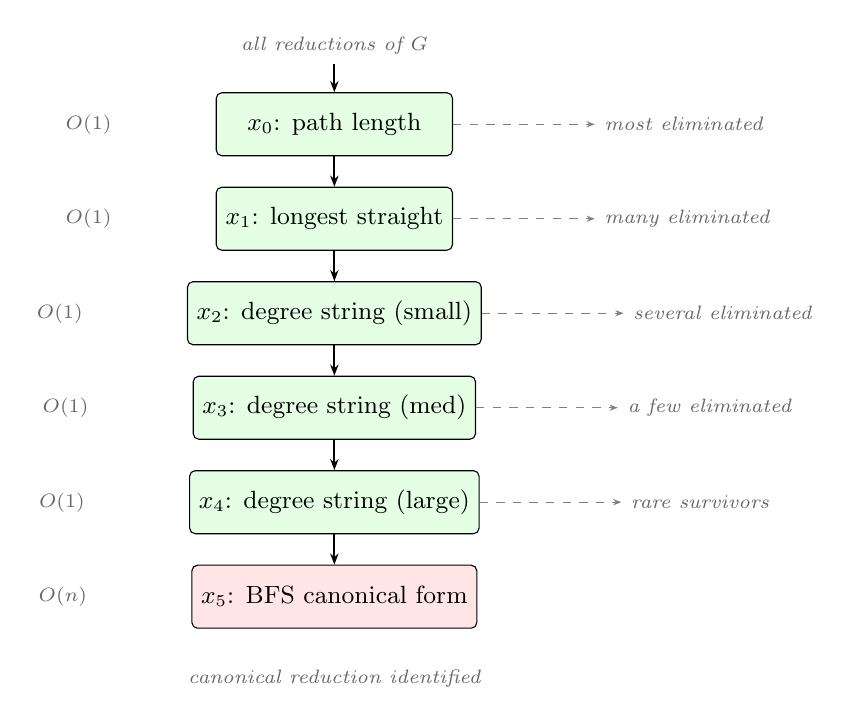
\begin{tikzpicture}[
    % --- Styles ---
    stage/.style={draw, rounded corners=2pt, minimum width=30mm,
                  minimum height=8mm, align=center, font=\small},
    cheap/.style={stage, fill=green!10},
    expensive/.style={stage, fill=red!10},
    count/.style={font=\scriptsize\itshape, text=black!60},
    elim/.style={-{Stealth[length=3pt]}, dashed, gray},
    surv/.style={-{Stealth[length=4pt]}, thick},
]

% === Stages top to bottom ===
\node[count] (alllabel) at (0, 5.5) {all reductions of $G$};
\node[cheap]     (x0) at (0, 4.5) {$x_0$: path length};
\node[cheap]     (x1) at (0, 3.3) {$x_1$: longest straight};
\node[cheap]     (x2) at (0, 2.1) {$x_2$: degree string (small)};
\node[cheap]     (x3) at (0, 0.9) {$x_3$: degree string (med)};
\node[cheap]     (x4) at (0,-0.3) {$x_4$: degree string (large)};
\node[expensive] (x5) at (0,-1.5) {$x_5$: BFS canonical form};

% === Survivor arrows (downward) ===
\draw[surv] (alllabel) -- (x0);
\draw[surv] (x0) -- (x1);
\draw[surv] (x1) -- (x2);
\draw[surv] (x2) -- (x3);
\draw[surv] (x3) -- (x4);
\draw[surv] (x4) -- (x5);

% === Eliminated reductions (arrows to the right) ===
\node[count, right=18mm of x0] (e0) {most eliminated};
\node[count, right=18mm of x1] (e1) {many eliminated};
\node[count, right=18mm of x2] (e2) {several eliminated};
\node[count, right=18mm of x3] (e3) {a few eliminated};
\node[count, right=18mm of x4] (e4) {rare survivors};

\draw[elim] (x0.east) -- (e0);
\draw[elim] (x1.east) -- (e1);
\draw[elim] (x2.east) -- (e2);
\draw[elim] (x3.east) -- (e3);
\draw[elim] (x4.east) -- (e4);

% === Cost annotations on the left ===
\node[count, left=12mm of x0] {$O(1)$};
\node[count, left=12mm of x1] {$O(1)$};
\node[count, left=12mm of x2] {$O(1)$};
\node[count, left=12mm of x3] {$O(1)$};
\node[count, left=12mm of x4] {$O(1)$};
\node[count, left=12mm of x5] {$O(n)$};

% === Result ===
\node[count, below=4mm of x5] {canonical reduction identified};

\end{tikzpicture}
\caption{The 6-tuple cascade.  All reductions enter at the top.  At
each stage, reductions whose $x_i$ value is not minimal are eliminated
(dashed arrows).  The expensive BFS canonical form ($x_5$, cost $O(n)$)
is computed only for the rare survivors of the $O(1)$ stages.  Lazy
evaluation in Haskell implements this short-circuiting automatically
via the derived \texttt{Ord} instance on tuples.}
\label{fig:sixtuple}
\end{figure}

%----------------------------------------------------------------------
\subsection{\texttt{isCanonical}: the acceptance test}
%----------------------------------------------------------------------

\begin{lstlisting}
isCanonical :: Expansion -> DualGraph -> Bool
isCanonical expansion g' =
    case canonicalReduction g' of
      Nothing          -> False  -- should not happen: g' is reducible
      Just (cRed, _)   -> inverse expansion `isEquivReduction` cRed
\end{lstlisting}

The expansion is accepted if and only if its inverse is the canonical
reduction of the result (or is equivalent to it under the automorphism
group).

\begin{lstlisting}
isEquivReduction :: Reduction -> Reduction -> Bool
isEquivReduction r1 r2 =
    redKind r1 == redKind r2 &&
    canonOrd r1 == canonOrd r2
\end{lstlisting}

%======================================================================
\section{Algebraic Properties Enabling Parallelism}
\label{sec:parallel}
%======================================================================

The functional decomposition exposes three properties that enable
safe parallelism without changing the algorithm's semantics.

%----------------------------------------------------------------------
\subsection{Independence}
%----------------------------------------------------------------------

\begin{proposition}[Subtree independence]
For distinct dual fullerenes $g_1 \neq g_2$:
\[
  \texttt{canonicalChildren}\; n\; g_1
  \quad\text{is independent of}\quad
  \texttt{canonicalChildren}\; n\; g_2
\]
There is no shared state, no side effects, and no communication
between subtree computations.
\end{proposition}

This follows directly from the purity of all five component functions.

\begin{figure}[ht]
\centering
% Parallel evaluation of the canonical parent forest.
% Each subtree is an independent unit of work.
% A spark depth controls the granularity of parallelism.
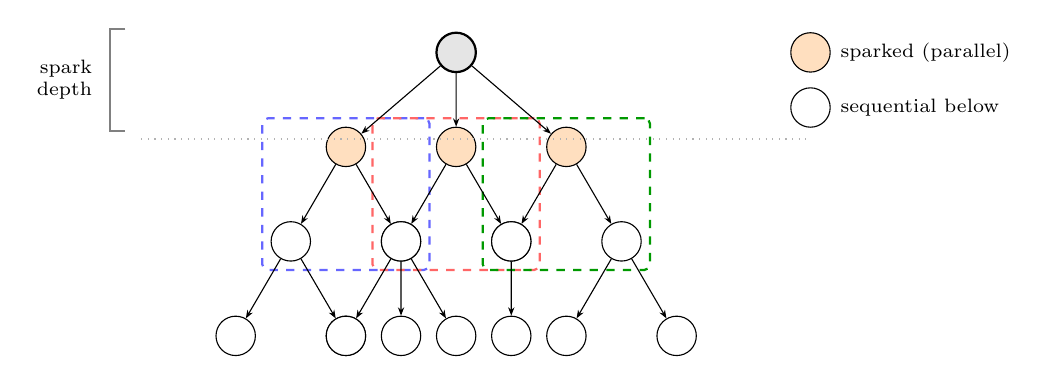
\begin{tikzpicture}[
    % --- Node styles ---
    gnode/.style={draw, circle, minimum size=5mm, font=\scriptsize},
    root/.style={gnode, thick, fill=black!10},
    sparked/.style={gnode, fill=orange!25},
    sequential/.style={gnode, fill=white},
    % --- Thread styles ---
    thread/.style={draw, thick, rounded corners=2pt, dashed},
    thread1/.style={thread, blue!60},
    thread2/.style={thread, red!60},
    thread3/.style={thread, green!60!black},
    thread4/.style={thread, purple!60},
    % --- Layout ---
    level distance=12mm,
    sibling distance=14mm,
    edge from parent/.style={draw, -{Stealth[length=3pt]}},
]

% === The tree ===
\node[root] (r) {}
  child { node[sparked] (a) {}
    child { node[sequential] (a1) {}
      child { node[sequential] {} }
      child { node[sequential] {} }
    }
    child { node[sequential] (a2) {}
      child { node[sequential] {} }
    }
  }
  child { node[sparked] (b) {}
    child { node[sequential] (b1) {}
      child { node[sequential] {} }
      child { node[sequential] {} }
    }
    child { node[sequential] (b2) {} }
  }
  child { node[sparked] (c) {}
    child { node[sequential] (c1) {}
      child { node[sequential] {} }
    }
    child { node[sequential] (c2) {}
      child { node[sequential] {} }
      child { node[sequential] {} }
    }
  };

% === Spark depth annotation ===
\draw[thick, black!50] (-4.2, 0.3) -- (-4.4, 0.3) -- (-4.4, -1.0) -- (-4.2, -1.0);
\node[font=\scriptsize, align=right, left] at (-4.5, -0.35) {spark\\depth};
\draw[dotted, black!30] (-4.0, -1.1) -- (4.5, -1.1);

% === Thread boxes around subtrees ===
\begin{scope}[on background layer]
  % Thread 1: subtree rooted at (a)
  \node[fit=(a)(a1)(a2), thread1, inner sep=3pt] {};
  % Thread 2: subtree rooted at (b)
  \node[fit=(b)(b1)(b2), thread2, inner sep=3pt] {};
  % Thread 3: subtree rooted at (c)
  \node[fit=(c)(c1)(c2), thread3, inner sep=3pt] {};
\end{scope}

% === Legend ===
\node[sparked, label={[font=\scriptsize]right:sparked (parallel)}]
  at (4.5, 0) {};
\node[sequential, label={[font=\scriptsize]right:sequential below}]
  at (4.5, -0.7) {};

\end{tikzpicture}
\caption{Parallel evaluation with depth-limited sparking.  Nodes above
the spark depth (orange) create parallel sparks; their subtrees
(dashed boxes) are evaluated by independent threads.  Below the spark
depth, evaluation is sequential.  The \texttt{using}/\texttt{Strategy}
annotation controls the spark depth without changing the algorithm.}
\label{fig:parallel}
\end{figure}

%----------------------------------------------------------------------
\subsection{Commutativity of result collection}
%----------------------------------------------------------------------

\begin{proposition}[Monoidal collection]
Results are collected via list concatenation, which is associative.
The set of fullerenes $\Ful(n)$ is independent of evaluation order:
\[
  \Ful(n) = \bigcup_{r \in \mathrm{roots}} \mathrm{leaves}_n(r)
\]
where $\mathrm{leaves}_n(r)$ denotes all nodes at the target size in
the subtree rooted at $r$.
\end{proposition}

%----------------------------------------------------------------------
\subsection{Parallel strategies}
%----------------------------------------------------------------------

Using Haskell's \texttt{Control.Parallel.Strategies}, parallelism is
expressed as an annotation that does not change the denotational
semantics:

\begin{lstlisting}
-- Sequential (reference implementation)
fullerenes :: Int -> [DualGraph]
fullerenes nTarget =
    concatMap flatten (generationForest nTarget)
  & filter (\g -> numVertices g == nTarget)

-- Parallel at the forest roots (coarse-grained)
fullerenesPar :: Int -> [DualGraph]
fullerenesPar nTarget =
    concatMap flatten trees
  & filter (\g -> numVertices g == nTarget)
  where
    trees = generationForest nTarget
              `using` parList (evalTree rseq)

-- Parallel with depth-limited sparking (fine-grained)
generationForestPar :: Int -> Int -> Forest DualGraph
generationForestPar nTarget sparkDepth =
    unfoldForest (stepPar sparkDepth) (seeds nTarget)

stepPar :: Int -> DualGraph -> (DualGraph, [DualGraph])
stepPar depth g
  | depth > 0 = children `using` parList rseq
  | otherwise  = children
  where children = canonicalChildren nTarget g
\end{lstlisting}

\begin{remark}
The \texttt{using} combinator has type
$a \to \texttt{Strategy}\;a \to a$ and is semantically the identity.
Replacing it with \texttt{const id} recovers the sequential version.
\end{remark}

%----------------------------------------------------------------------
\subsection{Type class abstraction}
%----------------------------------------------------------------------

The algorithm can be parameterised over the evaluation strategy using a
type class, allowing the same code to be interpreted as DFS, BFS, or
parallel evaluation:

\begin{lstlisting}
class Monad m => SearchMonad m where
  yield    :: DualGraph -> m ()      -- emit a result
  branch   :: [m a] -> m [a]         -- fork on children
  prune    :: Bool -> m ()           -- cut a subtree

-- DFS: m = []  (list monad)
-- BFS: m = Seq (sequence-based level-order)
-- Par: m = Eval or Par (parallel evaluation)
\end{lstlisting}

The core recursion becomes:

\begin{lstlisting}
generate :: SearchMonad m => Int -> DualGraph -> m ()
generate nTarget g = do
    when (numVertices g == nTarget) (yield g)
    let children = canonicalChildren nTarget g
    branch [generate nTarget c | c <- children]
    return ()
\end{lstlisting}

%======================================================================
\section{Pruning as Predicate Composition}
\label{sec:bounds}
%======================================================================

The bounding lemmas are the key to buckygen's performance.  In the
functional formulation, each lemma is a \emph{predicate} that bounds
the maximum useful expansion length.  Predicates compose via
\texttt{minimum} (meet in the lattice of natural numbers ordered by
$\le$).

%----------------------------------------------------------------------
\subsection{Individual bounds}
%----------------------------------------------------------------------

\begin{lstlisting}
type Bound = DualGraph -> Int -> MaxLength

-- Lemma 1: Non-IPR bound
-- Every reducible non-IPR dual fullerene has a reduction of length <= 2.
boundNonIPR :: Bound
boundNonIPR g _nTarget
  | hasAdjacentDeg5 g = 2   -- has L0 reduction, so children <= 2+2
  | otherwise          = maxBound

-- Lemma 2: Child bound
-- If g has a reduction of length d <= 2, children have length <= d+2.
boundChild :: Bound
boundChild g _nTarget =
    case shortestReductionLength g of
      Just d | d <= 2 -> d + 2
      _               -> maxBound

-- Lemma 3: L0 tightening
-- If g has an L0 reduction, all canonical children have length <= 2.
boundL0 :: Bound
boundL0 g _nTarget
  | hasL0Reduction g = 2
  | otherwise        = maxBound

-- Lemma 4: Three independent L1s
-- Three pairwise-disjoint L1 reductions => children have length <= 2.
boundThreeL1 :: Bound
boundThreeL1 g _nTarget
  | hasThreeIndepL1 g = 2
  | otherwise         = maxBound

-- Lemma 5: Geometric bound
-- Expansion of length d not canonical if result has < 12*f(floor((d-1)/2)) vertices.
boundGeometric :: Bound
boundGeometric _g nTarget = maxD
  where
    maxD = maximum [d | d <- [1..], vertexLowerBound d <= nTarget]
    vertexLowerBound d = 12 * f (div (d - 1) 2)
    f x = 1 + div (5 * x * (x + 1)) 2
\end{lstlisting}

%----------------------------------------------------------------------
\subsection{Composition}
%----------------------------------------------------------------------

\begin{lstlisting}
allBounds :: [Bound]
allBounds = [boundNonIPR, boundChild, boundL0, boundThreeL1, boundGeometric]

composeBounds :: [Bound] -> Bound
composeBounds bs g n = minimum [b g n | b <- bs]
\end{lstlisting}

\begin{figure}[ht]
\centering
% Bound composition: individual bounds feed into min, producing the tightest bound.
% This is a meet operation in the lattice (N, <=).
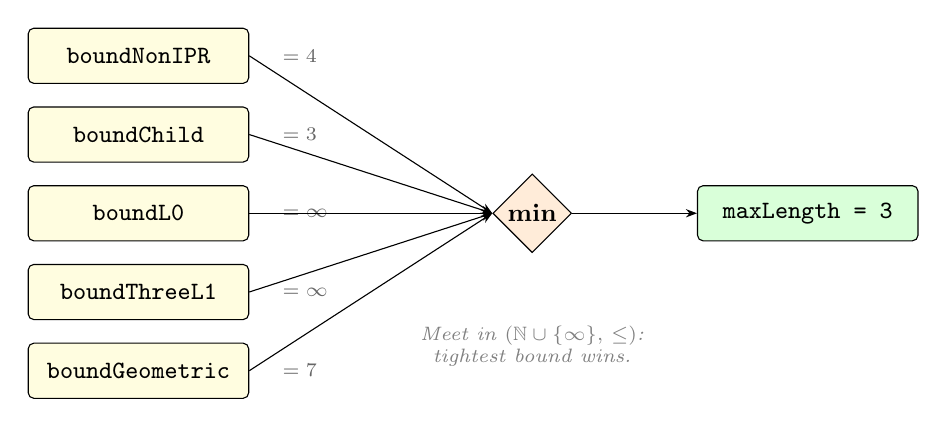
\begin{tikzpicture}[
    bound/.style={draw, rounded corners=2pt, minimum width=28mm,
                  minimum height=7mm, fill=yellow!12, font=\small\ttfamily},
    meet/.style={draw, diamond, minimum size=10mm, fill=orange!15,
                 font=\small\bfseries, inner sep=1pt},
    result/.style={draw, rounded corners=2pt, minimum width=28mm,
                   minimum height=7mm, fill=green!15, font=\small\ttfamily},
    flow/.style={-{Stealth[length=4pt]}},
    val/.style={font=\scriptsize, text=black!60},
]

% === Individual bounds (left column) ===
\node[bound] (b1) at (0, 4)   {boundNonIPR};
\node[bound] (b2) at (0, 3)   {boundChild};
\node[bound] (b3) at (0, 2)   {boundL0};
\node[bound] (b4) at (0, 1)   {boundThreeL1};
\node[bound] (b5) at (0, 0)   {boundGeometric};

% === Example values (right of each bound) ===
\node[val, right=3mm of b1] {$= 4$};
\node[val, right=3mm of b2] {$= 3$};
\node[val, right=3mm of b3] {$= \infty$};
\node[val, right=3mm of b4] {$= \infty$};
\node[val, right=3mm of b5] {$= 7$};

% === Meet (minimum) node ===
\node[meet] (min) at (5, 2) {min};

% === Result ===
\node[result] (out) at (8.5, 2) {maxLength = 3};

% === Arrows from bounds to meet ===
\foreach \b in {b1,b2,b3,b4,b5}
  \draw[flow] (\b.east) -- (min.west);

% === Arrow from meet to result ===
\draw[flow] (min.east) -- (out.west);

% === Annotation ===
\node[below=8mm of min, font=\scriptsize\itshape, text=black!50, align=center]
  {Meet in $(\mathbb{N} \cup \{\infty\},\, \le)$:\\
   tightest bound wins.};

\end{tikzpicture}
\caption{Bound composition.  Each bounding lemma independently computes
a maximum expansion length (or $\infty$ if inapplicable).  The
\texttt{composeBounds} function takes their minimum---the meet in the
lattice $(\mathbb{N} \cup \{\infty\}, \le)$.  New bounds (chemical,
geometric, symmetry) are added by appending to the list.  Example
values shown for a particular graph~$g$.}
\label{fig:bounds}
\end{figure}

\begin{proposition}[Soundness of composition]
If $b_1, \ldots, b_k$ are sound bounds (no canonical child is
excluded), then $\min(b_1, \ldots, b_k)$ is also sound.
\end{proposition}

\begin{proof}
If an expansion of length $\ell$ yields a canonical child, then
$\ell \le b_i(g, n)$ for all $i$.  Hence
$\ell \le \min_i b_i(g, n)$.
\end{proof}

%----------------------------------------------------------------------
\subsection{Extensibility}
%----------------------------------------------------------------------

New pruning criteria---chemical, geometric, or symmetry-based---are
simply new elements of the \texttt{[Bound]} list:

\begin{lstlisting}
-- Example: IPR bound (no adjacent pentagons in result)
boundIPR :: Bound
boundIPR g _nTarget
  | hasL0Reduction g = 0     -- L0 always creates adjacent pentagons
  | otherwise        = maxBound

-- Example: minimum pentagon distance >= k
boundPentagonDistance :: Int -> Bound
boundPentagonDistance k g nTarget = ...

-- Compose all bounds including new ones
myBounds :: [Bound]
myBounds = allBounds ++ [boundIPR, boundPentagonDistance 3]
\end{lstlisting}

%======================================================================
\section{Branch-and-Bound Extension}
\label{sec:branchbound}
%======================================================================

For optimisation problems over fullerenes (e.g.\ finding the most
stable isomer), the generation forest supports branch-and-bound via a
shared bound that is monotonically tightened.

%----------------------------------------------------------------------
\subsection{The monotonicity requirement}
%----------------------------------------------------------------------

\begin{definition}[Monotone bound]
A predicate $p : \texttt{DualGraph} \to \texttt{Bool}$ is
\textbf{monotone} with respect to the canonical parent forest if:
\[
  \neg\, p(G) \implies \neg\, p(G') \quad
  \text{for all descendants } G' \text{ of } G.
\]
That is, if a graph fails the bound, so do all its descendants.
\end{definition}

\begin{proposition}
If $p$ is monotone, pruning all subtrees where $p$ fails does not
miss any fullerene satisfying $p$.
\end{proposition}

%----------------------------------------------------------------------
\subsection{Impure communication of global bound}
%----------------------------------------------------------------------

Branch-and-bound requires a shared mutable bound---the one impure part
of the algorithm:

\begin{lstlisting}
type GlobalBound = IORef Double

branchAndBound :: GlobalBound -> Int -> DualGraph -> IO [DualGraph]
branchAndBound bestRef nTarget g = do
    best <- readIORef bestRef
    let dominated = lowerBound g >= best   -- prune
    if dominated then return []
    else do
      let children = canonicalChildren nTarget g
      results <- concat <$> mapM (branchAndBound bestRef nTarget) children
      when (numVertices g == nTarget) $ do
        let val = objectiveFunction g
        modifyIORef bestRef (min val)
      return (if numVertices g == nTarget then g : results else results)
\end{lstlisting}

\begin{remark}
In a parallel setting, the \texttt{IORef} is replaced by an
\texttt{MVar} or \texttt{TVar} (STM).  Because the bound is
monotonically tightened (only decreases), the worst case of a stale
read is exploring a subtree that could have been pruned---never
missing a valid result.
\end{remark}

%----------------------------------------------------------------------
\subsection{Separation of concerns}
%----------------------------------------------------------------------

The branch-and-bound extension composes cleanly with the generation
algorithm:

\begin{lstlisting}
-- Pure generation (Section 3)
generate :: Int -> [DualGraph]

-- Pure filtering (post-hoc)
filterStable :: [DualGraph] -> [DualGraph]

-- Branch-and-bound (interleaved pruning)
generateBB :: GlobalBound -> Int -> IO [DualGraph]
\end{lstlisting}

The first two are pure; the third adds a single impure channel (the
global bound).  All three produce the same results when the bound
function is sound.

%======================================================================
\section{Summary: The Complete Pipeline}
\label{sec:summary}
%======================================================================

The full algorithm in one page:

\begin{lstlisting}
-- 1. Seeds: irreducible fullerenes
seeds :: Int -> [DualGraph]
seeds n = [c20] ++ [c28 | n >= 28] ++ [c30 | n >= 30]

-- 2. Bound: composable pruning predicates
maxLength :: DualGraph -> Int -> MaxLength
maxLength g n = composeBounds allBounds g n

-- 3. Expand: enumerate candidate expansions
expansions :: MaxLength -> DualGraph -> [Expansion]

-- 4. Apply: patch replacement (local graph surgery)
applyExpansion :: Expansion -> DualGraph -> DualGraph

-- 5. Test: canonical acceptance
isCanonical :: Expansion -> DualGraph -> Bool

-- 6. Recurse: unfold the forest
canonicalChildren :: Int -> DualGraph -> [DualGraph]
canonicalChildren nTarget g =
    [ g' | e <- expansions (maxLength g nTarget) g
         , let g' = applyExpansion e g
         , numVertices g' <= nTarget
         , isCanonical e g' ]

generationForest :: Int -> Forest DualGraph
generationForest n = unfoldForest (\g -> (g, canonicalChildren n g)) (seeds n)

-- 7. Collect: filter to target size
fullerenes :: Int -> [DualGraph]
fullerenes n = concatMap flatten (generationForest n)
             & filter (\g -> numVertices g == n)
\end{lstlisting}

\noindent
The pipeline is:
\[
  \texttt{seeds}
  \;\xrightarrow{\texttt{unfold}}\;
  \texttt{forest}
  \;\xrightarrow{\texttt{flatten}}\;
  \texttt{stream}
  \;\xrightarrow{\texttt{filter}}\;
  \Ful(n)
\]
At each node, the step function is:
\[
  \texttt{bound} \to \texttt{expansions} \to \texttt{apply}
  \to \texttt{isCanonical} \to \texttt{children}
\]
Every function is pure.  Parallelism is an annotation
(\texttt{Strategy}), not a structural change.  New pruning criteria
extend the \texttt{[Bound]} list.

\begin{thebibliography}{10}

\bibitem{brinkmann_12}
G.~Brinkmann, J.~Goedgebeur, and B.D.~McKay.
\newblock The generation of fullerenes.
\newblock {\em Journal of Chemical Information and Modeling}, 52(11):2910--2918, 2012.

\bibitem{hasheminezhad_08}
H.~Hasheminezhad, H.~Fleischner, and B.D.~McKay.
\newblock A universal set of growth operations for fullerenes.
\newblock {\em Chemical Physics Letters}, 464:118--121, 2008.

\bibitem{mckay_98}
B.D.~McKay.
\newblock Isomorph-free exhaustive generation.
\newblock {\em Journal of Algorithms}, 26:306--324, 1998.

\end{thebibliography}

\end{document}
